\renewcommand\thisdir{papers/rtas22a}
\tikzsetfigurename{rtas22a-}
\renewcommand\figdir{\thisdir/figs}

% Commands for this paper
% if the conflict with previously defined commands use \renewcommand
\newcommand{\ewhc}{EWHC}

%%% Math Commands
\newcommand{\Alifted}{\mathcal{L}}
\newcommand{\sos}{\mathrm{SOS}}


\paper[Deadline-Miss-Adaptive Controller Implementation]{Deadline-Miss-Adaptive Controller Implementation for Real-Time Control Systems}
\authors{Nils Vreman \and Claudio Mandrioli \and Anton Cervin}

\begin{abstract}
    The policy used to implement a control algorithm in a real-time system can significantly affect the quality of control.
    In this paper, we present a method to adapt the controller implementation, with the objective to improve the system's performance under real-time faults.
    Our method compensates for missing state updates by adapting the controller parameters according to the number of consecutively missed deadlines. 
    It extends the state-of-the-art by considering dynamic controllers, which have had limited coverage in previous literature.
    The adaptation mechanism can be precomputed offline, solely based on knowledge about the controller and not on the controlled plant. 
    The approach is indifferent to the control design, as well as to the scheduling policy, and can be automatically realised by the operating system, thus improving the robustness of the control system to intermittent and unexpected real-time faults.
    We develop a stochastic performance analysis method and apply it to both a real plant and numerous simulated plants to evaluate our adaptive controller.
    Complementary to the stochastic analysis, we also do worst-case stability analysis of the resulting system.
    The results confirm the conjuncture that the adaptive controller improves both the performance and robustness in the presence of deadline misses.
\end{abstract}

\vfill
Originally published in IEEE 28th Real-Time and Embedded Technology and Applications Symposium (2022). 
Reprinted with permission.
\newpage

\section{Introduction}
\label{sec:intro}
Robustness is an essential concern in the design of control systems; they must be able to reliably handle nonlinear effects, unmodeled dynamics and noise, as well as delays in signal transmissions and dropped packets.
A lesser known problem concerns the assessment of robustness to \emph{computational issues} when controllers are implemented as periodic tasks in cheap embedded platforms.
Such tasks are expected to execute with real-time guarantees, i.e., their execution must be completed before a well-defined \emph{deadline}, when the control output must be sent to the actuator.
However, it is common in practice~\cite{akesson2020empirical} that tasks do not always complete within their deadline, causing what is called a \emph{deadline miss}.
This may be caused by delays in computation and memory accesses, transient overloads, bugs and other issues.

A popular model to describe real-time systems allowing deadline misses is the \emph{weakly-hard} model~\cite{Bernat:2001}. 
Weakly-hard tasks feature constraints defining a maximum number of deadlines that can be missed (alternatively, a minimum number to be satisfied) in a given number of consecutive periods.
This model is also the focus of this work.
To analyse the effects on the controlled plant, it is necessary to specify also \emph{what happens when the miss is experienced}, both in terms of changes to the control signal and of actions taken to deal with the failed computation~\cite{Pazzaglia:2019}.
An instance that experiences a deadline miss can be allowed to continue executing until completion (and possibly used later), while in other applications it is stopped and discarded instead.

There is however a mismatch between the guarantees that can be obtained for real-time tasks and platforms~\cite{Ernst:2015,choi2019job}, and the analysis available for \emph{control} tasks under the weakly-hard model.
Fewer works deal with \emph{stability} analysis of weakly-hard real-time control tasks, often targeting specific use-cases. 
For instance, the analysis in~\cite{Maggio:2020} is limited to constraints specifying a maximum number of \emph{consecutive} deadline misses.
The results in \cite{Linsenmayer:2017,linsenmayer2020linear}, obtained for networked linear control systems having packet dropouts bounded using the weakly-hard model, can not be generalised for \emph{late completions} or \emph{sets} of weakly-hard constraints.
The authors of~\cite{liang2019security,liang2020leveraging} studied safety guarantees of weakly-hard controllers, considering a miss as a discarded computation with a known periodic pattern.
%
In \cite{huang2020saw, huang2019formal}, an over-approximation-based approach is proposed to check the safety of nonlinear weakly-hard systems, where misses are treated as discarded computations and the actuator holds its previous value.
Convergence rates (providing sufficient stability guarantees) are analysed in~\cite{Gaukler:2019a}.
A Lyapunov-based stability analysis of nonlinear weakly-hard systems is studied in~\cite{hertneck2021efficient}, with deadline misses treated as packet dropouts.
However, the state-of-the-art listed above lack generalisability to more expressive real-time implementations, such as different deadline miss models or handling strategies.

This paper aims at filling the gap, by providing a stability analysis that can be applied to a class of generic weakly-hard models and deadline miss handling strategies.
First, we formally extend the weakly-hard model to explicitly consider the strategy used to handle the miss events. 
By leveraging an automaton representation of the sequences allowed by (a set of) extended weakly-hard constraints, we use Kronecker lifting and the joint spectral radius to properly express its stability conditions.
Using the concept of constraint dominance, we prove analytic bounds on the stability of a weakly-hard system with respect to \emph{less dominant} constraints.
Finally, we analyse the stability of the resulting closed-loop systems using \code{SparseJSR}~\cite{sparsejsr}, which exploits the sparsity pattern that naturally arises in the Kronecker lifted representation.
The proposed analysis calls for modularity and separation of concern, and can be a useful tool to decouple the constraint specification and the control verification.
%, the embedded system designer can extract a set of constraints to be used in the design phase, and the control engineer can verify that the proposed constraints satisfy all control requirements. 


\section{System Model}
\label{sec:sys-model}
\begin{figure}
    \centerline{\begin{tikzpicture}
\small
\node[draw] (ctrler) at (0,0) {
    \begin{tikzpicture}[
    task/.style={draw,
                 thick,
                 minimum width=3.2cm,
                 minimum height=1.8cm,
                 fill=white,
                 node distance =1.3cm},
    >=stealth]
        \node[] (hw) at (0,0) {\textbf{ECU}};
        \node[task, below of=hw, yshift=6, xshift=-7, opacity=.3] (task-3) [align=center]{};
        \node[task, below of=hw, yshift=4, xshift=-5, opacity=.5] (task-2) [align=center]{};
        \node[task, below of=hw, yshift=2, xshift=-3, opacity=.7] (task-1) [align=center]{};
        \node[task, below of=hw, yshift=-1] (task-c)[align=left]{Control Task $\ctrler$ \\[0.5mm]
                                                    \small
                                                      \texttt{y = read\_input();}\\
                                                      \texttt{u = ctrl\_comp();}\\
                                                      \texttt{write\_output(u);}};
    \end{tikzpicture}
};

\node[draw,minimum height=2cm] (plant) at (5,0) [align=center]{
    Physical Plant $\plant$ \\[1mm]
    $\begin{aligned}
    x_{t+1} &= \Ap x_t \!+\! \Bp u_t \!+\! \Wp w_t\\
    y_t &= \Cp x_t \!+\! \Dp u_t 
    \end{aligned}$
};

\draw[->] ([yshift=-0.5cm] plant.west) -- node[yshift=-0.2cm]{$y$} ([yshift=-0.5cm]ctrler.east);
\draw[->] ([yshift= 0.5cm]ctrler.east) -- node[yshift=0.2cm]{$u$} ([yshift= 0.5cm] plant.west);
\draw[->]([yshift=0.8cm]plant.north)--node[xshift=0.2cm]{$w$}(plant);

\end{tikzpicture}
}
    \caption{Typical structure of a computer-controlled system. \emph{Left:} the Electronic Control Unit (ECU) implementing a real-time system, including a task executing the controller. \emph{Right:} the physical plant controlled by the actuation variable $u$, affected by the disturbance $w$, and producing the measurement~$y$.}
    \label{fig:ctrl-loop}
\end{figure}

This section introduces the necessary background and models needed for the remainder of the paper.
We discuss the real-time implementation of a general linear controller and how it can affect the performance of the system. 
We start by describing the behaviour of the system under \emph{ideal} conditions. 
Based on this, we state how \emph{deadline misses} in the real-time implementation affect the system's behaviour.

\subsection{Control Systems under Ideal Operations}
The objective of a control system is to regulate a physical process, usually called a \emph{plant}, so that it behaves as desired. 
Figure~\ref{fig:ctrl-loop} shows the structure of a control system, where an Electronic Control Unit (ECU) implements a real-time system. 
Among the different tasks executed in the system, there is a task responsible for the control computations, denoted as the control task.
Every job released by this task performs the following actions:
\begin{enumerate*}[label=(\roman*)]
    \item Read measurements from the sensors.
    \item Use the sensor information to update its state and compute a control action. 
    \item Write the control action to the actuators.
\end{enumerate*}
The executed algorithm is generally designed using control theory, where the effective application of the algorithm relies on assumptions about the real-time execution.  

The dynamic behaviour of a plant is commonly described using a state-space model~\cite{Astrom:2008}. 
Such models are constituted of two sets of equations: one describing the dynamics of the plant and another one describing the relation between the plant state and the available measurements. 
Describing physical phenomena, those equations are for the most part continuous and nonlinear. 
However, for control design and implementation purposes, they are commonly transformed into a discrete-time linear time-invariant (LTI) state-space model:
\begin{equation}
    \label{eq:plant}
    \plant: \,\, \left\{
    \begin{aligned}
        x_{k+1} &= \Ap\,x_k + \Bp\,u_k + \Wp\,w_k \\
        y_k &= \Cp\,x_k + \Dp\,u_k 
    \end{aligned}
    \right.
\end{equation}
Here, the variable $k$ counts the number of discrete time steps that have passed since the system started executing. 
Furthermore, the variable $x_k \in \R^{n_x}$ represents the \emph{plant state}, $u_k \in \R^{n_u}$ corresponds to the \emph{control signal} computed in order to affect the plant, $w_k \in \R^{n_w}$ models disturbances and reference signals, and $y_k \in \R^{n_y}$ is the \emph{measurement signal} available to the controller. 
For what concerns the matrices, $\Ap \in \R^{n_x \times n_x}$ captures the relation between the current state and the next state, while $\Bp \in \R^{n_x \times n_u}$ and $\Wp \in \R^{n_x \times n_w}$ respectively capture how the control signal and the exogenous signals affect the state at the next time step.
Furthermore, $\Cp \in \R^{n_y \times n_x}$ and $\Dp \in \R^{n_y \times n_u}$ respectively describe how the current state and control signal relate to the measurements.

To control the behaviour of the plant, a \emph{controller} $\ctrler$ is synthesised to follow some desired properties, such as: 
\begin{enumerate*}[label=(\roman*)]
    \item stability, 
    \item speed of convergence, 
    \item control effort, and 
    \item disturbance rejection.
\end{enumerate*}
The stability requirement enforces that none of the signals diverge and is a necessary condition for all controllers.
Moreover, a controller that fulfils all requirements will make the output converge to the reference value within a specified time, while minimising the control effort and the effect of possible disturbances.

Controllers are commonly implemented as fixed-rate, periodically executing tasks, following the Logical Execution Time (LET) paradigm~\cite{Henzinger:2003,Kirsch:2012, Ernst:2018}.
Adopting this paradigm, the sensors are read at the beginning of the task period, and the control action is written to the actuators at the end of the period. 
This minimises the effect of fluctuations in the execution pattern of the control algorithm (called jitter) at the cost of introducing a one-step delay in the actuation.

While they are sometimes specified as transfer functions~\cite{Astrom:2008}, controllers are often \emph{implemented} as discrete-time state-space systems.
More specifically, we assume that the controller is an LTI system that takes the measurement $y_k$ as input and produces the control signal $u_{k+1}$ as output:\footnote{Note that we adopt a positive feedback convention.}
\begin{equation}
    \label{eq:ctrler}
    \ctrler: \,\, \left\{
    \begin{aligned}
        z_{k+1} &= \Ac\,z_k + \Bc\,y_k \\
        u_{k+1} &= \Cc\,z_{k} + \Dc\,y_k.
    \end{aligned}
    \right.
\end{equation}
Here, $z_k \in \R^{n_z}$ represents the internal state of the controller.
The second equation, specifying the control action at step $k+1$, captures the one-step delay introduced by the LET paradigm.
The matrices $\Ac \in \R^{n_z \times n_z}$, $\Bc \in \R^{n_z \times n_y}$, $\Cc \in \R^{n_u \times n_z}$, and $\Dc \in \R^{n_u \times n_y}$ govern the behaviour of the controller.

In conjunction with Equation~\eqref{eq:ctrler}, we define two types of controllers: \emph{static} and \emph{dynamic}.

\begin{definition}[Static Controller]%
    We denote a \emph{static controller} as any controller $\ctrler$ that is \emph{stateless} (i.e., it has no internal state $z$;\, $n_z = 0$).
\end{definition}

\begin{definition}[Dynamic Controller]%
    We denote a \emph{dynamic controller} as any controller $\ctrler$ that is \emph{stateful} (i.e., it has an internal state $z$;\, $n_z\geq 1$).
\end{definition}

From the definitions above, we note that a static controller can be written as a fixed gain matrix times the input (i.e., $\ctrler \,:\, u_{k+1} = \Dc y_k$), while a dynamic controller is equivalent to~\eqref{eq:ctrler} with non-empty matrices $\Ac$, $\Bc$, $\Cc$, and $\Dc$.
Examples of static controllers include proportional (P) controllers, state feedback controllers, and linear--quadratic regulators (LQR), while dynamic controllers include proportional--integral--derivative (PID) controllers, lead--lag compensators, and linear--quadratic--Gaussian (LQG) regulators~\cite{Astrom:2008}.

\subsection{Control Systems Subject to Deadline Misses}

We assume that the controller $\ctrler$ is implemented as a periodic task with period $\Ts$ and implicit deadlines. 
Intuitively, each execution period of the control task corresponds to one time step $k$.
At the start of period $k$, the task releases a \emph{job} that should be completed before the deadline at time $(k+1) \Ts$.

Faults in the real-time system can affect the timely execution of the control task~\cite{Steinbauer:2013}.
We denote the outcome of a job's execution as either a deadline \emph{hit} or \emph{miss}, corresponding to whether the job completed its execution before its deadline or not. 
The source of a deadline miss could be a temporary CPU overload~\cite{Baruah:1997}, cache misses~\cite{Milligan:1996, Wang:2012},  or unexpected preemption from hardware interrupts or higher priority tasks~\cite{Stankovic:1995}.
However, the analysis and adaptation methods presented in this paper are independent of the origin of the deadline miss.

To study what happens when the controller misses a deadline, we have to define how the system behaves in such circumstances.
In particular, three aspects need to be considered: 
\begin{enumerate*}[label=(\roman*)]
    \item how the controller state is updated, 
    \item how the actuator handles the lack of a new control signal~\cite{Schenato:2009}, and
    \item how the operating system handles a job that misses its deadline~\cite{Pazzaglia:2019, Cervin:2005}.
\end{enumerate*}
The first item refers to what happens to the internal state $z$ when the controller is unable to finish its execution ahead of its dedicated deadline.
Henceforth, we assume that when the controller misses its deadline, the controller state is \emph{not} updated (implying $z_{k+1} = z_k$). 
This is motivated by the possibility to roll back $z_k$ to a previous state~\cite{akesson:2020, Seong:2001, Zhang:2003} and by the impossibility to guarantee that the state update was finished if the job was only partially completed.

Regarding the second item, mainly two actuator models have previously been considered in the literature: \emph{\tZ{}} and \emph{\tH{}} \cite{Schenato:2009}.
Under the \tZ{} model, if the job released at time $k\Ts$ misses its deadline at time  $(k+1)\Ts$, the actuator outputs $u_{k+1} = 0$.
This strategy is uncommon in practice, because it performs well only in very specific cases~\cite{Vreman:2021ecrts}. 
Instead, the more common actuator model is to hold the control signal in the case of a missed deadline: $u_{k+1} = u_k$.
Although our proposed adaptation is in itself independent of the actuator model, the \tH{} model has been adopted in the analysis and examples of this paper.

% For the final item, there exists at least three different employable strategies dealing with missed deadlines: 
For what concerns the handling of the job that missed the deadline, there exist at least three different employable strategies:
\begin{enumerate*}[label=(\alph*)] % roman already used for the three aspects
    \item \emph{\tK{}}
    \item \emph{\tS{}}, and 
    \item \emph{\tQ{}}.
\end{enumerate*}
When using the \tK{} strategy, the job that missed its deadline gets terminated, the controller state is rolled back, and the next job is released. 
The \tS{} strategy does not terminate the job that missed its deadline. 
Instead, it lets the job continue its execution, not releasing subsequent jobs until the active one has finished executing.
\tQ{} behaves similarly to the \tS{} strategy: it does not kill the current job, but it does release the subsequent jobs to the job queue.
Both the \tS{} and \tQ{} strategies allow jobs to work with outdated input data, since they do not terminate jobs that miss their deadline.
Thus, they introduce a lag in the actuation of the control law, which in most cases reduces the control performance with respect to what could be achieved with the \tK{} strategy.

For the remainder of this paper we will use the \tK{} strategy, since it
\begin{enumerate*}[label=(\alph*)]
    \item introduces explicit breakpoints in which to adapt the controller,
    \item supplies the controller with the latest sensor measurement after an overrun,
    \item helps free computational resources in overrun situations, and
    \item is a common choice in both industry and literature~\cite{akesson:2020, Bernat:2001, Hertneck:2019}.
\end{enumerate*}
Furthermore, we note that in~\cite{Vreman:2021ecrts} it has been observed that the actuator model is of greater relevance than the handling of the deadline overrun.
We also note that an effective implementation of the \tK{} strategy that includes state roll-back requires the implementation of checkpointing mechanisms~\cite{Zhang:2003,Seong:2001}, which might not be implemented by default in a real-time system.

We conclude this section by mentioning that various models have been proposed to describe tasks
that may experience deadline misses, e.g., soft~\cite{Marchand:2008} or weakly hard models~\cite{Bernat:2001, hammadeh:2017}.
For the adaptive controller in this work, we only assume that the number of consecutive deadline misses $\counter$ is bounded by a finite quantity $\counter_{max} < \infty$.
This assumption is a practical necessity, since accepting an infinite run of deadline misses would completely disconnect the plant from the controller~\cite{Maggio:2020}.

Solely for performance analysis, in Section~IV-B we adopt a stochastic model of the sequences of deadline hits and misses. 
Such a model can be computed from a probabilistic task set model using existing techniques~\cite{Chen:2017, Chen:2018, markovic:2021}. 
However, we remark that the proposed adaptive controller implementation is independent of the stochastic deadline miss model.

\subsection{Control System Stability under Deadline Misses}
\label{sec:stability}
Guaranteeing the stability of control systems is essential in control engineering.
A linear control system without exogenous inputs is \emph{stable} if and only if the system's state always converges to zero irrespective of its initial value.
Assuming ideal conditions, i.e., no deadline misses, stability can be verified by checking whether all the closed-loop system's eigenvalues lie inside the unit circle.
However, in the presence of deadline misses, the classical stability criteria are no longer sufficient, since the dynamics of the control system is time-varying and changes according to the specific pattern of deadline misses.
For such cases, switched system stability analysis (also known as switching stability) is a viable extension of classical stability~\cite{Liberzon:2003}.
In this paper, we analyse the switching stability using both a time-averaged (Markov Jump Linear Analysis~\cite{Fang:2002}) and a worst-case (Joint Spectral Radius~\cite{Rota:1960}) approach.

Modelling the deadline misses as a stationary random process with known statistical properties allows us to calculate an analytical time-averaged performance index of the closed-loop system.
If the performance index is finite, then the system is guaranteed to be stable in the mean-square sense (meaning that the state will not diverge with probability~1).
We develop our approach to compute the time-averaged performance in Section~\ref{sec:analysis}.

If the statistical properties of the deadline misses are unknown or uncertain, switching stability can still be analysed under worst-case conditions.
The Joint Spectral Radius (JSR) generalises the spectral radius of a matrix (i.e., the largest absolute eigenvalue) to a set of matrices; thus, the JSR characterises the largest asymptotic growth (or contraction) rate of the states. % arbitrary matrix product of the matrices in the set.
If the JSR of the set of closed-loop matrices representing $i = \{0,1,\ldots,\counter_{max}\}$ deadline misses (followed by a hit) is below $1$ then the system is switching stable.
Conversely, if it is above $1$, there exists at least one sequence of deadline misses and hits that makes the system unstable.
There exist both toolboxes and methods for calculating the JSR for control systems subject to deadline misses~\cite{Jungers:2014, Maggio:2020, Vreman:2021}.


\section{Problem Description}
\label{sec:problem-descr}
The work presented in this paper is closely related to two broad research areas, namely, the analysis of 
\begin{enumerate*}[label=(\roman*)]
    \item weakly hard systems and
    \item fault-tolerant control systems.
\end{enumerate*}

\textbf{Weakly Hard Systems:}
Deadline misses can be seen as sporadic events caused by
unforeseen delays in the system. Such delays could for instance
be induced by overload activations~\cite{Xu:2015, Ernst:2014}
or cache misses~\cite{Altmeyer:2014, Davis:2013}. The idea behind
weakly hard analysis is that deadline misses are permitted under
predefined constraints. Such systems have been analysed
extensively from a real-time scheduling
perspective~\cite{Bernat:1997, Caccamo:1997, Choi:2019,
Hammadeh:2019}.  The weakly hard models have gained traction in
the research community as a tool to understand and analyse
systems with sporadic faults~\cite{Soudbakhsh:2013, Bund:2014,
Frehse:2014, Bund:2015, Hammadeh:2017a, Hammadeh:2017b, Sun:2017,
Ahrendts:2018, Soudbakhsh:2018, Pazzaglia:2018,
Gaukler:2019a}. In a recent paper, Gujarati et
al.~\cite{Gujarati:2019} analysed and compared different methods
for estimating the overall reliability of control systems using
the weakly hard task model. Furthermore, the authors
of~\cite{Broman:2019} proposed a toolchain for analysing the
strongest, satisfied weakly hard constraints as a function of the
worst-case execution time.

\textbf{Fault-Tolerant Control Systems:} 
Real-time systems are sensitive to faults. Due to their
safety-critical nature, it is arguably more important
to guarantee fault-tolerance with respect to other
classes of systems. Some of these faults can be
described using the weakly hard model. Due to the
nature of control systems, special analysis techniques
can combine fault models and the physical characteristics of
systems.

Fault-tolerance has been investigated in
many of its aspects, e.g., fault-aware scheduling 
algorithms~\cite{Rowe:2013, Buttazzo:2000b} and the analysis of systems with unreliable components~\cite{Teich:2015}. Furthermore, 
restart-based design~\cite{Caccamo:2017a, Caccamo:2018} has been used as a technique to guarantee resilience. The fault models are frequently assumed to target overload-prone 
systems, or systems with components subject to sporadic failures. Bursts of faults have been observed to affect real systems~\cite{Phan:2015, Vreman:2020}.
Gujarati et al.~\cite{Gujarati:2018} proposed an analysis 
method for networked control systems that uses active replication and quantifies the resilience of the control
system to stochastic errors. 
Maggio et al.~\cite{Maggio:2020} developed a tool for determining the stability of a control system where the control task behaves according to the weakly hard 
model. From the control perspective, there has been extensive research into both analysis and mitigation of real-time faults in feedback systems~\cite{Ramanathan:1997, Chakraborty:2014b, Chakraborty:2018}. Very often, this research produced tools to analyse the effect of computational delays~\cite{Cervin:2019} and of choosing specific scheduling policies or parameters~\cite{Palopoli:2000, Cervin:2005}, possibly including deadline misses. In a few instances, researchers looked at how to improve the performance of control systems in conjunction with scheduling information~\cite{Buttazzo:2007}. One such effort analyses modifications to the code of classic and simple control systems to handle overruns that reset the period of execution of the control task~\cite{Pazzaglia:2021}.
Abdi et al.~\cite{Caccamo:2017b} proposed a control design method for safe system-level restart, mitigating 
unknown faults during runtime execution, while keeping the system inside a safe operating space. 
Pazzaglia et al.~\cite{Pazzaglia:2019} used the scenario theory to derive a control design method accounting for potential 
deadline misses, and discussed the effect of different deadline handling strategies.
Linsenmayer et al.~\cite{Linsenmayer:2020} worked on the stabilisation of weakly-hard linear control systems for networked control systems, with some extension for nonlinear systems~\cite{Hertneck:2019}. In the considered setup, faults compromise network transmissions, but do not interfere with the controller computation (assuming that the computation is triggered). The work also focused on stability, with no control performance evaluation.

To the best of our knowledge, no previous work has devised a combined stability and performance analysis to understand how faults (even when they can be tolerated) affect the plant that should be controlled when different deadline handling strategies are used.



\section{Real-Time Controller Adaptation}
\label{sec:darc}
In this section, we derive an adaptive implementation scheme for real-time controllers to address the problems discussed in Section~\ref{sec:problem-form}.
We explain the intuition behind the proposed adaptation; then, starting from an arbitrary linear control algorithm, we show how to derive the adapted controller.
The adaptive controller is complemented with a probabilistic analysis method to evaluate its effectiveness for a given control system and a given deadline miss model.

\subsection{Adaptive Controller Synthesis}%
\label{sec:adaptation}%
%
To simplify and generalise the adaptation approach, we do not assume any information about the control design, apart from the controller itself. 
In practice, this implies that we consider neither the specific control design technique, the control system requirements, nor the plant's dynamics.
The controller is assumed to be given in state-space form, specified by~\eqref{eq:ctrler}.
This assumption is made without loss of generality, since any realisable linear digital controller can be expressed in this form~\cite{Astrom:2008}.

%ideal controller
The controller behaves \emph{ideally} when every control period includes one job completing the execution of Equation~\eqref{eq:ctrler}, i.e., every job hits its deadline.
By iterating the equation, the desired controller state and control action at any future time step can be computed. 
We formally define this behaviour as follows:

\begin{definition}[Ideal Controller]%
    We denote the \emph{ideal controller}, $\ctrler\funof{\counter}$, as the discrete-time LTI controller $\ctrler$ evolved over an interval of $\counter+1$ consecutive deadline hits.
    The controller state and output at the end of the interval are
    \begin{equation}
        \label{eq:ctrler-ideal}
        \ctrler\funof{\counter}:\,\, 
        \left\{\begin{aligned}
            z_{k+\counter+1} &= \Ac^{\counter+1}\,z_{k} + \textstyle\sum_{i=0}^{\counter} \Ac^i \Bc \,y_{k+\counter-i}\\
            u_{k+q+1} &= \Cc\, \Ac^{q}\,\,z_k + \\
            &\hspace{-2em}+ \Cc\, \textstyle\sum\nolimits_{i=1}^{q}\, \left[ \Ac^{i-1}\, \Bc\, y_{k+q-i}\right] 
            + \Dc\, y_{k+q}.
        \end{aligned}\right.
    \end{equation}
\end{definition}
With $\counter=0$ we obtain the ideal controller behaviour over a single time step.

From the definition above, we see how the quantities of interest, $z$ and $u$, are computed using the values of $y$ in the interval $\left[ k, k+\counter \right]$. 
These values correspond to the periodic measurements coming from the sensors.
%
In the presence of deadline misses, the control task discards the measurements and does not update the controller's state.
Thus, both the state and output of the controller deviate from their desired behaviours. 
Applying Equation~\eqref{eq:ctrler} to a scenario of $\counter$ consecutive deadline misses, we obtain the following:

\begin{definition}[Nominal Controller]%
    We denote the \emph{nominal controller}, $\ctrler^n\funof{\counter}$, as the discrete-time LTI controller $\ctrler$ evolved over an interval of $\counter$ consecutive deadline misses followed by one deadline hit. 
    After the hit, the state and output are given by
    \begin{equation}
        \label{eq:ctrler-miss}
        \ctrler^n\funof{\counter}:\,\, 
        \left\{\begin{aligned}
            z_{k+\counter+1} &= \Ac\,z_{k} + \Bc\,y_{k+\counter}\\
            u_{k+\counter+1} &= \Cc\,z_{k} + \Dc\,y_{k+\counter}.
        \end{aligned}\right.
    \end{equation}
    In the absence of deadline misses, we have $\ctrler^n\funof{0} = \ctrler$.
\end{definition}

By comparing \eqref{eq:ctrler-ideal} and~\eqref{eq:ctrler-miss} we see that, when deadline misses occur, the controller state $z_{k+\counter+1}$ and control action $u_{k+\counter+1}$ diverge from the ideal values, i.e., the ones that would be obtained in the presence of only deadline hits. 
To compensate for this error (and consequently minimise it), we propose to dynamically alter the controller's computations in real time according to the number of deadline misses. 

Ideally, we would like an adaptive controller $\ctrler^a\funof{\counter}$ that mimics the ideal controller $\ctrler\funof{\counter}$ for any $\counter$.
However, this is infeasible due to how the controller's dynamics evolves during an interval of deadline misses.
More specifically, Equation~\eqref{eq:ctrler-ideal} shows that $\ctrler\funof{\counter}$ depends on the values of $y_{k+i}$ for $i \in \left\{ 0, 1, \ldots, \counter-1 \right\}$.
When the control task is subjected to faults, the corresponding jobs $j_{k+i}$ miss their respective deadline. 
Thus, the unfinished jobs are terminated prematurely, a new job is released, and the corresponding measurement values $y_{k+i}$ are lost.
The nominal controller, after a series of misses, has access only to the sample $y_{k+\counter}$.
This fundamentally limits how well the controller's ideal behaviour can be reconstructed.

Hence, we propose the use of an interpolation scheme to minimise the effect of the lost measurement values.
We approximate the missing measurement values using a linear interpolation between $y_{k-1}$ and $y_{k+\counter}$ according to
%
\begin{equation}
    \label{eq:interpolation}
    \hat y_{k+\counter-i} = \frac{i\, y_{k-1} + (\counter+1-i)\, y_{k+\counter}}{\counter+1} .
\end{equation}
%
If we substitute the values of $y$ that are missing in the ideal controller, Equation~\eqref{eq:ctrler-ideal}, with the corresponding interpolated ones $\hat y$ from Equation~\eqref{eq:interpolation}, we obtain an adaptive controller as follows:

\begin{definition}[Adaptive Controller]%
    We denote the \emph{adaptive controller}, $\ctrler^a\funof{\counter}$, as an adaptation of the controller $\ctrler$ evolved over an interval of $\counter$ consecutive deadline misses followed by one deadline hit.
    After the hit, the state and output are
    \begin{equation}
        \label{eq:adaptive}
        \ctrler^a\funof{\counter}: \,\,
        \left\{
            \begin{aligned}
                z_{k+\counter+1} &= F_z(\counter)\,z_{k} +  F_y(\counter)\,y_{k-1} + G_y(\counter)\,y_{k+\counter} \\
                u_{k+\counter+1} &= H_z(\counter)\,z_{k} + H_y(\counter)\,y_{k-1} + K_y(\counter)\,y_{k+\counter},
            \end{aligned}\right.
    \end{equation}
    where
    \begin{equation*}
        \begin{aligned}
            \Ac_z(\counter) &= \Ac^{\counter+1} \\
            \Ac_y(\counter) &= \textstyle\sum\nolimits_{i=0}^{\counter}\, \tfrac{i}{\counter+1}\, \Ac^{i}\, \Bc \\
            \Bc_y(\counter) &= \textstyle\sum\nolimits_{i=0}^{\counter}\, \tfrac{\counter+1-i}{\counter+1}\, \Ac^{i}\, \Bc \\
            \Cc_z(\counter) &= \Cc\, \Ac^\counter \\
            \Cc_y(\counter) &= \Cc\, \textstyle\sum\nolimits_{i=1}^{\counter}\, \tfrac{i}{\counter+1}\, \Ac^{i-1}\, \Bc \\
            \Dc_y(\counter) &= \Dc + \Cc\, \textstyle\sum\nolimits_{i=1}^{\counter}\, \tfrac{\counter+1-i}{\counter+1}\, \Ac^{i-1}\, \Bc.
        \end{aligned}
    \end{equation*}
\end{definition}
Note that for $\counter = 0$ we recover the original controller.

All matrices in $\ctrler^a\funof{q}$ ($\counter \in \{0, \ldots, \counter_{max}\}$) can be precomputed and stored in memory.
Compared to the nominal controller, the two matrices $F_y$ and $H_y$ of size $n_z \times n_y$ and $n_u \times n_y$ need to be added to the controller, and one full set of controller matrices needs to be stored for each value of $\counter$.
The memory requirement thus grows linearly with $\counter_{max}$.
%the number $\counter$ of maximum tolerated misses.
%This is exactly $\counter_{max}$ times the size of the non-adaptive controller expanded with $F_y$ and $H_y$.
The adaptive controller also needs to store the old measurement value $y_{k-1}$, which makes it marginally more complex.

% How we overcome the limitations of previous work
We now briefly discuss how the limitations described in Section~\ref{sec:problem-form} are addressed.
This work proposes an adaptation of the $\Ac$, $\Bc$, $\Cc$, and $\Dc$ matrices of the controller, thus adapting also the \emph{dynamic} part of the controller.
The adaptive controller's matrices can be precomputed directly from the specified controller using Equation~\eqref{eq:adaptive}, and then stored in memory for each $\counter \leq \counter_{max}$.
The control algorithm can be developed independently of this adaptation, hence no extra design effort is needed.
For $\counter=0$ the adaptive and the ideal controllers are equivalent, i.e., $\ctrler^a\funof{0} = \ctrler\funof{0}$, thus guaranteeing that the controller's performance is not degraded under ideal conditions.
Concerning the limitation of increased runtime overhead, each time a job is released, the counter $\counter$ of immediately preceding deadline misses is evaluated and the corresponding controller matrices are selected.
Hence, the execution time of the adaptive controller will be independent of $\counter$ and only marginally longer than for the nominal controller.

\begin{figure}[tp!]
    \centerline{\def \ada {\figdir/example-figs/adaptive.csv}
\def \lqg {\figdir/example-figs/lqg.csv}
\def \nom {\figdir/example-figs/lqg-nominal.csv}

\begin{tikzpicture}
    \footnotesize

    %Main axes
    \begin{axis}[%
            height=\timeplotheight,
            width=\columnwidth,
            xmin=0,
            xmax=5,
            ymin=-0.4,
            ymax=1.1,
            xlabel={Time (s)}, 
            ylabel={State},
            ytick={-0.4,-0.2,0,0.2,0.4,0.6,0.8,1.0,1.2},
            yticklabels={-0.4,-0.2,0,0.2,0.4,0.6,0.8,1.0,1.2},
            ylabel near ticks,
            grid=major,
            grid style={dashed,black!20},
            legend cell align=left,
            scatter/classes={a={mark=x, mark size=3, color=misscolour}},
            % legend columns = 2
            ]
        
        % LQG x
        \addplot[lqgnomcolour, solid, very thick] table[x=T, y=X, col sep=comma] {\nom};
        
        % LQG x
        \addplot[lqgcolour, dash pattern={on 7pt off 2pt}, very thick] table[x=T, y=X, col sep=comma] {\lqg};
        
        % Ada x
        \addplot[adacolour, dash pattern={on 7pt off 2pt}, very thick] table[x=T, y=X, col sep=comma] {\ada};
        
        % Misses
        % scatter src=explicit symbolic gets the scatter definition in axis options.
        \addplot+[scatter, only marks, thick, scatter src=explicit symbolic] coordinates{
            (0.3, -0.4) [a]
            (0.7, -0.4) [a]
            (0.9, -0.4) [a]
            (1.6, -0.4) [a]
            (2.1, -0.4) [a]
            (2.2, -0.4) [a]
            (2.3, -0.4) [a]
            (2.9, -0.4) [a]
            (3.2, -0.4) [a]
            (3.5, -0.4) [a]
            (3.8, -0.4) [a]
            (4.1, -0.4) [a]
            (5.0, -0.4) [a]
        };
        
        % Legend
        \legend{$x_2$ ($\ctrler_2 $ -- ideal), $x_2$ ($\ctrler^n_2 $ -- nominal), $x_2$ ($\ctrler^a_2 $ -- adaptive), Overrun};
    \end{axis}

\end{tikzpicture}
}
    \caption{The state $x_2$ corresponding to $\plant$ being controlled by the LQG controller $\ctrler_2$ (dashed green) or adaptive LQG (dashed orange) controller during an interval of sporadic overloads ($\times$).
    The corresponding ideal behaviour (system not subject to overruns, solid green) is also plotted.}
    \label{fig:lqgs-lqgd}
\end{figure}

In Section~\ref{sec:problem-form}, we presented a motivating example of why it is insufficient to analyse static controllers subject to overruns.
We conclude this section with a continuation of this example showing the benefits of our scheme.

\begin{example}[Application to Motivating Example]%
    Consider the plant $\plant$, from Equation~\eqref{eq:example-plant}, controlled by the LQG controller $\ctrler_2$.
    We apply our proposed scheme to $\ctrler_2$, obtaining the corresponding adaptive controller $\ctrler_2^a\funof{\counter}$.
    In Figure~\ref{fig:lqgs-lqgd}, we compare the plant state obtained by controlling the plant using the two controllers, subject to the same deadline misses as in Figure~\ref{fig:lqr-lqg}.
    The dashed green line and the dashed orange line correspond, respectively, to the nominal LQG (the same as in Figure~\ref{fig:lqr-lqg}) and adaptive LQG.
    The solid green line corresponds to the ideal controller's behaviour, i.e., in the absence of deadline misses.
    We note a significant improvement in the performance of the adaptive LQG compared to the nominal LQG: the oscillations disappear and the state converges faster.
\end{example}

The proposed adaptive controller is inspired by the ideal controller $\ctrler\funof{\counter}$, % not subjected to deadline misses.
but there is no a priori guarantee that it will perform better than the nominal controller $\ctrler^n\funof{\counter}$. 
However, for a given plant and deadline miss model, the closed-loop system can be analysed and compared for different controllers. 
Since the actual sequence of hits and misses is generally unpredictable, in the next section, we propose a probabilistic method to compare the performance of the adaptive controller with the nominal controller.

\subsection{Stochastic Performance Analysis}
\label{sec:analysis}
To analyse the performance of the closed-loop system, we need to model the plant, the external disturbance $w$, and the sequences of deadline misses.
For what concerns the plant, we consider the standard state-space model presented in Equation~\eqref{eq:plant}.
The plant disturbance $w$ and the sequence of deadline hits and misses are modelled as stationary random processes with known statistical properties.
This allows us to analyse the time-averaged performance of the closed-loop system subject to deadline misses.
The analysis offered here is inspired by~\cite{Nilsson:1998}, which in turn relies on classical results for jump linear systems~\cite{Blair:1975}.

The control performance is measured in terms of the weighted stationary variance of the plant output $y$,
\begin{equation}
    \label{eq:cost}
    J = \E{ y_k^{\T} Q y_k },
\end{equation}
where $Q \in \R^{n_y \times n_y}$ is a positive semidefinite weighting matrix\footnote{Without loss of generality, we assume that zero is the desired plant output. A non-zero reference value can be modelled as an exogenous signal that is stored in the plant and offset in the measurement signal.}.
A smaller value of the cost $J$ is better, as it means that the controller can suppress the disturbance $w$ more effectively.
Additionally, the closed loop is guaranteed to be \emph{stable} in the mean-square sense as long as $J$ is finite~\cite{Fang:2002}, i.e., $J < \infty$.

The state of the complete system consists of the plant and the controller in feedback interconnection, together with the buffered previous measurement value and the calculated next control signal.
Accordingly, we define the closed-loop state vector as
\begin{equation*}
    \tilde{x}_k = \begin{bmatrix} x_k \\ z_k \\ y_{k-1} \\ u_k \end{bmatrix} .
\end{equation*}
As seen in Figure~\ref{fig:ctrl-loop}, the only external input of the closed-loop system is the disturbance $w$.
Hence, the state of the closed loop evolves according to the time-varying linear system
\begin{equation}
    \label{eq:cl-system}
    \tilde{x}_{k+1} = \Phi_{k} \tilde{x}_k + \Gamma w_k.
\end{equation}
Here,
\begin{equation*}
    \Gamma = \begin{bmatrix} \Wp \\ 0_{(n_z+n_y+n_u) \times n_w} \end{bmatrix},
\end{equation*}
while $\Phi_k$ can be either $\Phi_{hit}(\counter)$ or $\Phi_{miss}$, depending on whether the current deadline was hit or missed, and defined as\fix{Consider changing $\Phi$ here to match other papers.}
\begin{equation*}
    \Phi_{hit}(\counter) = \begin{bmatrix} \Ap & 0 & 0 & \Bp \\
        \Bc_y(\counter) \, \Cp & \Ac_z(\counter) & \Ac_y(\counter) & \Bc_y(\counter) \, \Dp \\
        \Cp & 0 & 0 & \Dp \\
        \Dc_y(\counter) \, \Cp & \Cc_z(\counter) & \Cc_y(\counter) & \Dc_y(\counter) \, \Dp
    \end{bmatrix},
\end{equation*}
where $\counter$ denotes the number of consecutive deadline misses since the last hit, and
\begin{equation*}
    \Phi_{miss} = \begin{bmatrix} \Ap & 0 & 0 & \Bp \\
        0 & I_{n_z} & 0 & 0 \\
        0 & 0 & I_{n_y} & 0 \\
    0 & 0 & 0 & I_{n_u} \end{bmatrix}.
\end{equation*}

Assuming that $w$ is a zero-mean white noise process with known covariance matrix $R = \E{w_k \cdot w_k^{\T}} \in \R^{n_w \times n_w}$, we can calculate how the state covariance, $P_k = \E{\tilde{x}_k\cdot \tilde{x}_k^{\T}}$, evolves over time.
Evaluating the covariance of both sides in Equation~\eqref{eq:cl-system} we obtain (see, e.g., \cite{AstWit:1984})
\begin{equation}
    \label{eq:covariance}
    P_{k+1} = \Phi_k P_k \Phi_k^{\T} + \Gamma R \Gamma^{\T} .
\end{equation}

\begin{figure}[t]
    \centerline{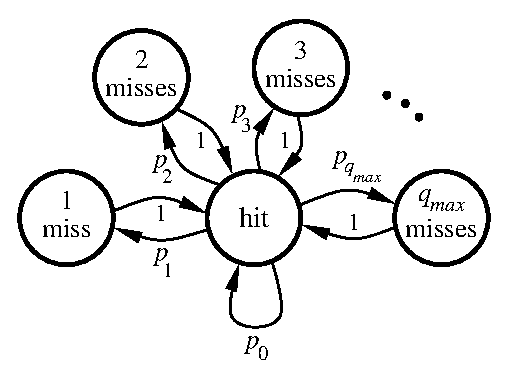
\includegraphics[scale=0.7]{\figdir/misses.eps}}
    \caption{Markov model for the random sequence of hits and misses.}
    \label{fig:Markov}
\end{figure}

We model the task execution as a random process, assuming that the pattern of hits and misses in the real-time system is described by the homogeneous Markov model shown in Figure~\ref{fig:Markov}.
In this model, after each hit, the system will experience a miss interval of length $\counter \in \{0,\ldots,\counter_{max}\}$ with independent probability $p_\counter$. Naturally, $\sum_{i=0}^{\counter_{max}} p_i = 1$.

In each interval, the system will experience $\counter$ deadline misses followed by one deadline hit. Iterating \eqref{eq:covariance} over said interval, the covariance will then develop as
\begin{equation*}
    \label{eq:intervalP}
    \begin{aligned}
        P_{k+q+1} &= \Phi_{hit}(\counter)  \Bigl((\Phi_{miss})^\counter P_k (\Phi_{miss}^{\T})^\counter \Bigr.\\
        &\Bigl.+ \textstyle\sum_{i=0}^{q-1} (\Phi_{miss})^i \Gamma R \Gamma^{\T} (\Phi_{miss}^{\T})^i \Bigr)\Phi_{hit}^{\T}(\counter)  \\
        &+ \Gamma R \Gamma^{\T} .
    \end{aligned}
\end{equation*}
The time-varying closed-loop system together with the Markov model define a \emph{discrete-time Markov jump linear system} for which well-established results exist (e.g., \cite{Blair:1975,Nilsson:1998,Lincoln:2002}). Using this theory, it is possible to calculate the \emph{stationary} (time-averaged) state covariance, denoted $\overbar{P}$. With this, the performance \eqref{eq:cost} can finally be obtained as
\begin{equation*}
    J = \trace{ \overbar{P} \, \overbar{Q} },
\end{equation*}
where
\begin{equation*}
    \overbar{Q} = \begin{bmatrix}
        C^{\T}Q C & 0 \\ 0 & 0_{n_z+n_y+n_u}
    \end{bmatrix}.
\end{equation*}

To compare the performance of different implementations, we first define the \emph{ideal performance} as the cost $J$ obtained when there are no deadline misses (i.e., $p_0 = 1$ and $p_i = 0$, $i \geq 1$).
We then obtain the \emph{relative performance degradation} of an arbitrary controller $\ctrler^{\dagger}$ by calculating the weighted mean-square difference between the actual and ideal systems' outputs, $y^{\dagger}_k$ and $y_k$ respectively, and normalising it with respect to the ideal performance $J$:
\begin{equation}
    \label{eq:relcost}
    \frac{\Delta J^{\dagger}}{J} = \frac{\E{ (y^{\dagger}_k - y_k)^{\T} Q (y^{\dagger}_k - y_k) }}{ \E{ y_k^{\T} Q y_k }}.
\end{equation}
This can be found by analysing both systems in parallel when driven by the same noise sequence $w_k$:
\begin{equation*}
    \begin{bmatrix}
        \tilde{x}_{k+1}^\dagger \\ \tilde{x}_{k+1}%^b 
    \end{bmatrix} =
    \begin{bmatrix}
        \Phi_k^\dagger & 0 \\ 0 & \Phi_k%^b
    \end{bmatrix}
    \begin{bmatrix}
        \tilde{x}_k^\dagger \\ \tilde{x}_k%^b 
    \end{bmatrix} +
    \begin{bmatrix}
        \Gamma \\ \Gamma
    \end{bmatrix} w_k
\end{equation*}
After finding the stationary state covariance $\overbar{P}_e$ of this extended system (using the same technique as referred to above), we can retrieve the absolute performance difference as
\begin{equation*}
    \label{eq:deltaJ}
    \Delta J^{\dagger} = \trace{ \overbar{P}_e  \begin{bmatrix}
        \phantom{-}\overbar{Q} & -\overbar{Q}\phantom{,} \\
        -\overbar{Q} & \phantom{-}\overbar{Q}\phantom{,}
    \end{bmatrix} }.
\end{equation*}



\section{Experimental Evaluation}
\label{sec:results}
%
In this section, we compare our adaptive controller with the nominal controller implementation for different case studies.
We demonstrate the practical usefulness of the proposed controller by examining its impact on real hardware, namely, a ball and beam plant.
We compare the performance of the adaptive control system with the nominal one, according to the analysis presented in Section~\ref{sec:analysis}.
Finally, we complement the results with a worst-case switching stability analysis of the nominal and adaptive controlled systems.

In addition to the evaluation on the physical system, we present aggregate results obtained from a set of control benchmarks, representative of the process industry. %~\cite{Astrom:2004}.
We use this set of plants to evaluate the general applicability of our approach.
To make the evaluation comprehensive, we chose an unstable plant (the ball and beam) for the physical experiments and a set of mainly stable plants for the aggregate results.
Furthermore, we remark that all the considered controllers are dynamic.
As discussed in Section~\ref{sec:related}, to the best of our knowledge, only one previous work considers dynamic controllers~\cite{Pazzaglia:2021}.
In that work, however, a different overrun handling method is used, and a proper comparison is therefore not possible.

\subsection{Real World Evaluation -- Ball and Beam}
\label{sec:realplant}
%
\subsubsection*{System Description and Models}
The ball and beam~\cite{Wellstead:1978} is a common example in the automatic control literature and education, where a ball is free to roll over a beam that in turn is tilted by a servo motor.
The control objective is to make the ball position follow a reference trajectory across the beam by adjusting the voltage sent to the motor. Both the beam angle and the ball position can be measured.
Assuming the sampling period $\Ts = 0.01$~s, a discrete-time plant model $\plant$ was derived as
%
\begin{equation*}
\setlength\arraycolsep{1.25pt}
    \label{eq:bnb-plant}
    \plant : 
    \left\{
    \begin{matrix}
        x_{k+1} &=& 
        \begin{bmatrix}
            1 & 0.015 & 0.0003 & 0\\
            0 & 1 & 0.045 & 0\\
            0 & 0 & 1 & 0 \\
            0 & 0 & 0 & 1
        \end{bmatrix}\,x_k &+ 
        \begin{bmatrix}
            2.9\!\cdot\!10^{-5} \\
            0.0058 \\
            0.256 \\
            0
        \end{bmatrix}\,u_k + w_k \\ \vspace{-3mm} \\
        y_k &=& 
        \begin{bmatrix}
            0.5 & 0 & 0 & -1\\
            0 & 0 & 0.25 & 0
        \end{bmatrix}\,x_k, & 
    \end{matrix}
    \right.
\end{equation*}
where the four components of $x_k$ represent the ball position, ball velocity, beam velocity, and ball reference, respectively. The external signal vector $w_k$ is assumed to be white noise with variance $R = \diag{1,1,1,1}$. Under this state-space model, the objective is to regulate both outputs $y_k$ to zero, with the performance weighting matrix $Q = \diag{1,1}$.

To control $\plant$ we design a cascaded P--PID controller.
Cascaded controllers are frequently applied to systems with multiple measurements where one measured quantity affects another, but not vice versa.
Thus, the plant measurements can be controlled in sequential order (hence the naming \emph{cascaded}) using a controller designed for each measurement signal.
In our case study, this is implemented by a proportional (P) controller designed for controlling the beam's angle and a proportional--integral--derivative (PID) controller for the ball's position.
The controller is run as a periodically executing task with period $\Ts=0.01$~s on a single core CPU where overrun deadlines are killed and the corresponding sensor data is discarded. 
In between actuator calls, the control signal is assumed to be held constant.
The state-space representation of our controller is
%
\begin{equation*}
\setlength\arraycolsep{2pt}
    \label{eq:bnb-ctrler}
    \ctrler : \,\,
    \left\{
    \begin{aligned}
        z_{k+1} &= 
        \begin{bmatrix}
            1 & 0  \\
            0 & 0.9685 \\
        \end{bmatrix}\,z_k + 
        \begin{bmatrix}
            0.025 & 0 \\
            -0.2608 & 0
        \end{bmatrix}\,y_k, \\ \vspace{-4mm} \\
        u_{k+1} &= 
        \begin{bmatrix}
            -0.108 & -0.2608
        \end{bmatrix}\,z_k +
        \begin{bmatrix}
            -2.43 & -3
        \end{bmatrix}\,y_k.
        \end{aligned}
    \right.
\end{equation*}

\begin{table}[t]
    \centering
    \caption{Analytical study of the relative performance degradation of the ball and beam plant $\plant$ using either the nominal $\ctrler^n$ or adaptive controller $\ctrler^a$.}
    \renewcommand{\arraystretch}{1.6}
    \setlength{\tabcolsep}{5pt}
    \begin{tabular}{c | a b a b a b a} \hline
        $p$ & 10\% & 20\% & 30\% & 40\% & 50\% & 60\% & 70\% \\ \hline\hline
        ${\large\sfrac{\Delta J^n}{J}}$ & 2.5\% & 9.2\% & 20.8\% & 39.9\% & 75.3\% & 156\% & 452\% \\ \hline
        ${\large\sfrac{\Delta J^a}{J}}$ & 0.1\% & 0.1\% & 0.3\% & 0.6\% & 1.1\% & 2.5\% & 6.7\% \\ \hline
    \end{tabular}
    \label{tab:cost-sim}
\end{table}


\subsubsection*{Experiments Design}
We apply the performance analysis presented in Section~\ref{sec:analysis} to the plant model $\plant$ controlled using either the ideal ($\ctrler$), nominal ($\ctrler^n$), or adaptive ($\ctrler^a$) implementations from Section~\ref{sec:adaptation}.
We include the effect of deadline misses only on the nominal and adaptive control systems.
The probability distribution $p_\counter$ can be chosen arbitrarily according to the desired task model. 
For simplicity, we assume here that the deadline misses are Bernoulli distributed~\cite{Schenato:2007}, i.e., the probabilities of missing deadlines in each period are independently and identically distributed with probability $p$.
This results in the probability $p_\counter = (1-p)p^\counter$ of $\counter$ consecutive deadline misses followed by a hit.
We assume that no more than $\counter_{max}=20$ consecutive deadlines can be missed.
The latter assumption might seem restrictive, but if the probability of missing a deadline is $30\%$, the probability of missing $20$ consecutive deadlines is less than $4\cdot10^{-11}$.

\begin{table}[t]
    \centering
    \caption{Empirical study of the relative performance degradation of the real ball and beam plant using either the nominal $\ctrler^n$ or adaptive controller $\ctrler^a$.}
    \renewcommand{\arraystretch}{1.6}
    \setlength{\tabcolsep}{5pt}
    \begin{tabular}{c | a b a b a b a} \hline
        $p$ & 10\% & 20\% & 30\% & 40\% & 50\% & 60\% & 70\% \\ \hline\hline
        ${\large\sfrac{\Delta J^n}{J}}$ & 6.3\% & 27.1\% & 22.5\% & 50.5\% & 73.1\% & 260\% & $\infty$ \\ \hline
        ${\large\sfrac{\Delta J^a}{J}}$ & 6.1\% & 7.8\% & 3.2\% & 4.6\% & 3.8\% & 4.9\% & 11.7\% \\ \hline
    \end{tabular}
    \label{tab:cost-real}
\end{table}

\begin{figure}
    \centering
    \begin{tikzpicture}
\begin{groupplot}[%
    group style={group size = 1 by 1,
                 vertical sep = 0.25cm,
                 horizontal sep = 0.75cm},
    width = \columnwidth,
    height = 3.5cm,
    xmin=  500, xmax= 550,
    ymin= -1, ymax= 4,
    ytick = {0,1,2,3},
    title style = {yshift=-0.1cm},
    ylabel style = {yshift=-0.5cm},
    grid style = {dashed, black!20},
    grid = major,
    ]

    %%%%%%%%%%%%%%%%%%%%%%
    %% ideal controller %%
    %%%%%%%%%%%%%%%%%%%%%%
    \nextgroupplot[xlabel={Time (s)},
                   xlabel near ticks,
                   ylabel = {Pos. (cm)},
                   yticklabels = {0,5,10,15}, 
                   ylabel style = {yshift = 10pt},
                   title={Ball Position with the Ideal Controller $\ctrler$}
                  ]
    \addplot[smooth, thick, lqrnomcolour]
            table[col sep=comma, x=T, y=Y1]
            {\figdir/evaluation/ball-and-beam/data/experiment_M_10_P_50_Mode_1.csv};
    % reference plot
    \addplot[]coordinates {(500, 0)(525, 0)(525, 3)(550, 3)};

\end{groupplot}
\end{tikzpicture}

    \caption{Snippet of the test performed on the real ball and beam plant using the ideal controller, i.e., without deadline misses.
        The plot shows one period of the square wave used as reference, the black line. The blue line shows the ball's position.}
    \label{fig:real-plant-ideal}
\end{figure}


\begin{figure*}
    \centering
    \begin{tikzpicture}
\begin{groupplot}[%
    group style={group size = 1 by 4,
                 vertical sep = 0.6cm,
                 horizontal sep = 0.75cm},
    width = \columnwidth,
    height = 4.76cm,
    xmin=  500, xmax= 550,
    ymin= -0.75, ymax= 4,
    ytick = {0,1,2,3},
    title style = {yshift=-0.1cm},
    grid style = {dashed, black!20},
    grid = major,
    ]

    %%%%%%%%%%%%%%%%%%%%%%%%%%%%%%
    %% p=0.3 nominal controller %%
    %%%%%%%%%%%%%%%%%%%%%%%%%%%%%%
    \nextgroupplot[ylabel = {Pos. (cm)},
                   ylabel style = {yshift = -3pt},
                   ylabel right = {$\ctrler^n $},
                   xticklabels={},
                   yticklabels = {0,5,10,15}, ]
    \addplot[smooth, thick, lqgcolour,]
            table[col sep=comma, x=T, y=Y1]
            {\figdir/evaluation/ball-and-beam/data/experiment_M_20_P_30_Mode_2.csv};
    % reference plot
    \addplot[]coordinates {(500, 0)(525, 0)(525, 3)(550, 3)};
    \node[draw, fill=white] at (axis cs:545, 0) {$\rho=30\%$};

    %%%%%%%%%%%%%%%%%%%%%%%%%%%%%%%
    %% p=0.3 adaptive controller %%
    %%%%%%%%%%%%%%%%%%%%%%%%%%%%%%%
    \nextgroupplot[ylabel = {Pos. (cm)},
                   ylabel style = {yshift = -3pt},
                   ylabel right = {$\ctrler^a $},
                   xticklabels={},
                   yticklabels = {0,5,10,15}, ]
    \addplot[smooth, thick, adacolour,]
            table[col sep=comma, x=T, y=Y1]
            {\figdir/evaluation/ball-and-beam/data/experiment_M_20_P_30_Mode_3.csv};
    % reference plot
    \addplot[]coordinates {(500, 0)(525, 0)(525, 3)(550, 3)};
    \node[draw, fill=white] at (axis cs:545, 0) {$\rho=30\%$};

    %%%%%%%%%%%%%%%%%%%%%%%%%%%%%%
    %% p=0.5 nominal controller %%
    %%%%%%%%%%%%%%%%%%%%%%%%%%%%%%
    \nextgroupplot[xticklabels={},
                   yticklabels = {0,5,10,15},
                   ylabel = {Pos. (cm)},
                   ylabel style = {yshift = -3pt},
                   ylabel right = {$\ctrler^n $}, ]
    \addplot[smooth, thick, lqgcolour,]
            table[col sep=comma, x=T, y=Y1]
            {\figdir/evaluation/ball-and-beam/data/experiment_M_20_P_50_Mode_2.csv};
    % reference plot
    \addplot[]coordinates {(500, 0)(525, 0)(525, 3)(550, 3)};
    \node[draw, fill=white] at (axis cs:545, 0) {$\rho=50\%$};

    %%%%%%%%%%%%%%%%%%%%%%%%%%%%%%%
    %% p=0.5 adaptive controller %%
    %%%%%%%%%%%%%%%%%%%%%%%%%%%%%%%
    \nextgroupplot[xlabel = {Time (s)},
                   xlabel near ticks,
                   ylabel = {Pos. (cm)},
                   ylabel style = {yshift = -3pt},
                   ylabel right = {$\ctrler^a $},
                   yticklabels = {0,5,10,15}, ]
    \addplot[smooth, thick, adacolour,]
            table[col sep=comma, x=T, y=Y1]
            {\figdir/evaluation/ball-and-beam/data/experiment_M_20_P_50_Mode_3.csv};
    % reference plot
    \addplot[]coordinates {(500, 0)(525, 0)(525, 3)(550, 3)};
    \node[draw, fill=white] at (axis cs:545, 0) {$\rho=50\%$};

\end{groupplot}
\end{tikzpicture}

    \vspace{-3mm}
    \caption{Snippets of the tests performed on the real ball and beam plant for $p=30\%$ (two left plots) and $p=50\%$ (two right plots).
        The plots show one period of the square wave used as reference, the black line.
        The coloured lines show the ball position, in green for the nominal controller (upper plots) and orange for the adaptive controller (lower plots).}
    \label{fig:real-plant}
\end{figure*}

% performance metric
We measure the relative performance of the nominal and adaptive controllers according to the quantity $\sfrac{\Delta J^\dagger}{J}$ in Equation~\eqref{eq:relcost}.
Since the mean-square deviation from the ideal controller is used to evaluate the relative performance, the \emph{optimal} achievable cost is $0$.
For the real system, we do not feed the system with white noise, but we expose the system to a repeatable exogenous signal in the form of periodic reference changes. 
Furthermore, we evaluate the relative performance degradation empirically from the measured signals using Equation~\eqref{eq:relcost}, with $\mathbb{E}$ being interpreted as the mean value of the real signals.

To complement the performance analysis, we perform a JSR stability analysis on the model to determine the maximum number of consecutive deadline misses that are tolerated while still guaranteeing closed-loop stability.

\subsubsection*{Analytical Evaluation}
The performance results obtained with the analytical study of $\plant$ for different values of $p$ are summarised in Table~\ref{tab:cost-sim}.
From the table, we can see that the adaptive controller drastically improves the relative performance (in comparison to the nominal controller) across all deadline miss probabilities.
Already for small probabilities, the nominal controller significantly degrades the relative performance compared to the ideal controller; e.g., for $p = 30\%$ the relative performance is degraded by $20.8\%$. This can be compared to the  adaptive controller, where the relative performance reduction stays below $5\%$ until the miss probability reaches $70\%$.

Analysing the switching stability, we calculated the JSR for the set of closed-loop matrices corresponding to $i = \{0,1,\ldots,q\}$ consecutive deadline misses followed by one hit ($q \leq q_{max}$).
The nominal control system is guaranteed to be switching stable (i.e., the JSR is below $1$) for a maximum of $q=2$ consecutive deadline misses, while the adaptive control system is guaranteed stable up to $q=8$. 
We conclude that the adaptive controller improves also worst-case robustness against deadline misses for the ball and beam.
However, we emphasise that these results do \emph{not} imply that the system will go unstable if more deadline misses occurs; only that the system is \emph{guaranteed} switching stable if no more than $q$ consecutive deadline misses are ever experienced.

\subsubsection*{Empirical Evaluation}
We conducted experiments on the physical ball and beam plant to evaluate the performance of the controller on a real system.\footnote{A video, showing experiments with the real ball and beam system can be viewed at \texttt{https://youtu.be/6y\_C7NIzXto}. The video provides a real-world comparison between the nominal and adaptive controllers for $p = \left\{30\%, 50\%, 70\%\right\}$.}
Each experiment is run for $10$ minutes, where the control objective is for the ball to follow a square-wave reference across the beam.
The square wave has a period of $50$~s and alternates between position $0$ and $15$~cm.
Differently from the analytical evaluation, it is impossible to obtain the same exogenous signal $w_k$ in the different experiments.
While the reference changes can be exactly repeated, the real stochastic disturbances (in the form of electrical noise, mechanical glitches, etc.) are not repeatable.
This means that the empirical cost relative to the ideal case, as measured by Equation~\eqref{eq:relcost}, is not expected to be zero even in the complete absence of deadline misses.

Figure~\ref{fig:real-plant-ideal} displays a snippet of the ball's position (blue line) under said ideal conditions.
The ball quite successfully follows the reference (black line). 
Here, the fluctuations around the reference are caused by measurement noise and irregularities in the beam surface, where the latter can cause the ball to get lodged in an undesired position and thus result in oscillations.

After measuring the performance of the ideal controller, each controller ($\ctrler^n$ and $\ctrler^a$) was applied to the system, using probabilities $p \in \left\{ 10\%,\, 20\%,\, \ldots,\, 70\% \right\}$ of missing each deadline (with $\counter_{max} = 20$).
The results of the experiments are reported in Table~\ref{tab:cost-real}, where the relative performance degradation $\sfrac{\Delta J^\dagger}{J}$ is computed for both the nominal and adaptive controllers.
To give an intuition for how the physical system behaves, in Figure~\ref{fig:real-plant} we provide a snippet of a time plot portraying the ball's position controlled by either the nominal (upper plots) or adaptive (lower plots) controller.
We distinguish the differences between the nominal and adaptive controllers for a probability $p = 30\%$ (left plots) of missing a deadline.
The nominal controller shows oscillations around the reference value.
When the probability of missing a deadline is increased to $p = 50\%$ (right plots), the nominal controller's oscillations grow more evident, while the adaptive controller appears unaffected (compared to the ideal controller in Figure~\ref{fig:real-plant-ideal}).

% experiments comments
From Table~\ref{tab:cost-real}, we observe that the adaptive controller has a lower performance degradation across all deadline miss probabilities $p \geq 20\%$ compared to the nominal controller.
The performance of the adaptive controller seems virtually unaffected for $p \leq 60\%$, where the baseline relative degradation of approximately  $4\%$ to $8\%$ is due to the natural disturbances in the system.
The nominal controller on the other hand experiences significant performance degradation at higher miss probabilities, and for $p = 70\%$ the system becomes unstable -- we report this as an infinite cost.

In summary, both the analytical and empirical studies show that the adaptive controller $\ctrler^a$ consistently outperforms the nominal controller $\ctrler^n$ for the ball and beam. Furthermore, the adaptive controller can tolerate
a large likelihood of random deadline misses (at least $60\%$) without any noticeable performance degradation.

\subsection{Benchmark Evaluation -- Process Industry}
\label{sec:aggregate}
%
\subsubsection*{System Description and Models}
To evaluate the general applicability of the proposed adaptive controller, we perform an extensive evaluation campaign on a benchmark set of plants.
The set was developed specifically to evaluate various PID designs~\cite{Astrom:2004} in the process industry.
It consists of $134$ unique plants separated into $9$ categories, where each category has its own specific properties frequently recognised in the process industry.
Since the benchmark was developed specifically with process industrial plants in mind, the majority of the plants are stable, i.e., all their eigenvalues lie inside the unit circle.
However, there are also plants with integrating dynamics included in the benchmark, i.e., an eigenvalue in $1$; these plants are generally not considered stable.
For each plant, two controllers -- a PI and a PID controller -- are optimised using known methods~\cite{Garpinger:2008}; hence, $268$ unique control systems are analysed in total.

\subsubsection*{Experiments Design}
Similarly to the ball and beam, we analyse the relative performance of the nominal and adaptive controllers in accordance with the analysis described in Section~\ref{sec:analysis}.
We again consider the probability of missing a deadline to follow a Bernoulli distribution with probabilities $p \in \left\{ 10\%,\, 30\%,\, 50\%,\, 70\% \right\}$ and a maximum of $\counter_{max} = 20$ consecutive deadline misses.
We feed the systems with a stochastic disturbance and analytically evaluate the ability of the controllers to reject it.
Differently from the ball and beam, we analyse the systems when subject to brown noise, i.e., integrated white noise~\cite{Schmidt:1985}.
The brown noise model is generally considered appropriate for process industrial plants since it is dominant for low frequencies (e.g., load disturbances and disturbances from nearby heavy machinery).
We assume that the \emph{same} disturbance process enters the ideal, nominal, and adaptive control systems; this guarantees an unbiased comparison between the different controllers.
For each of the $268$ control systems we calculate the relative performance $\sfrac{\Delta J^\dagger}{J}$ for both the nominal and the adaptive controller.

Similarly to the ball and beam, we complement our performance analysis with a JSR worst-case stability analysis.

\begin{figure}
    \centering
    % Set number of bins for histograms in commands file

\begin{tikzpicture}
\begin{groupplot}[group style = {group size = 1 by 4,
                                 vertical sep=0.4cm},
                  width=\textwidth,
                  grid=both,
                  grid style={dashed,black!20},
                  height=2.8cm,
                  width=\columnwidth,
                  xmin=-5, xmax=2.2,
                  ymin=0, ymax=165,
                  tick align=inside,
                 ]

    %%%%%%%%%%%%%%%
    %%% p = 0.1 %%%
    %%%%%%%%%%%%%%%
    \nextgroupplot[xticklabels = {},
                   legend style = {at = {(0.5,1.1)},
                                   anchor = south,
                                   /tikz/every even column/.append style = {column sep=0.2cm}},
                   legend columns = 3
                  ]
        \addplot[ybar, ybar legend,
                 fill=lqgcolour,
                ] coordinates {(0,0)};
        \addlegendentry{Nominal}
        \addplot[ybar,
                 hist={bins=\binsaggregatedhist},
                 fill=lqgcolour,
                 forget plot,
                ] 
                table [y index=0, col sep=comma] 
                {figs/rtas22a/data/batch-results-10-log.csv};
        \addplot[ybar, ybar legend,
                 fill=adacolour,
                ] coordinates {(0,0)};
        \addlegendentry{Adaptive}
        \addplot[ybar, ybar legend,
                 hist={bins=\binsaggregatedhist},
                 fill=adacolour,
                 forget plot,
                ]
                table [y index=1, col sep=comma] 
                {figs/rtas22a/data/batch-results-10-log.csv};
        % \addlegendentry{$\mathcal{C}^{a}$}
        \addplot[red, dashed, ultra thick] coordinates {(2,0) (2,200)};
        \addlegendentry{Instability threshold}
        \node[draw, fill=white] at (axis cs:1, 115) {$\rho=10\%$};
    
    %%%%%%%%%%%%%%%
    %%% p = 0.3 %%%
    %%%%%%%%%%%%%%%
    \nextgroupplot[xticklabels= {},
                  ]
        \addplot[ybar, hist={bins=\binsaggregatedhist},
                 fill=lqgcolour,
                ] 
                table [y index=0, col sep=comma] 
                {figs/rtas22a/data/batch-results-30-log.csv};
        \addplot[ybar, hist={bins=\binsaggregatedhist},
                 fill=adacolour,
                ]
                table [y index=1, col sep=comma] 
                {figs/rtas22a/data/batch-results-30-log.csv};
        \draw[red,ultra thick, dashed] (axis cs:2,0)--(axis cs:2,200);
        \node[draw, fill=white] at (axis cs:1, 115) {$\rho=30\%$};

    %%%%%%%%%%%%%%%
    %%% p = 0.5 %%%
    %%%%%%%%%%%%%%%
    \nextgroupplot[xticklabels= {},
                   ylabel = {Number of systems},
                   ylabel near ticks,
                   ylabel style = {xshift=1cm},
                  ]
        \addplot[ybar, hist = {bins=\binsaggregatedhist},
                 fill = lqgcolour,
                ] 
                table [y index = 0, col sep = comma] 
                {figs/rtas22a/data/batch-results-50-log.csv};
        \addplot[ybar, hist={bins=\binsaggregatedhist},
                 fill=adacolour,
                ]
                table [y index=1, col sep=comma] 
                {figs/rtas22a/data/batch-results-50-log.csv};
        \draw[red,ultra thick, dashed] (axis cs:2,0)--(axis cs:2,200);
        \node[draw, fill=white] at (axis cs:1, 115) {$\rho=50\%$};

    %%%%%%%%%%%%%%%
    %%% p = 0.7 %%%
    %%%%%%%%%%%%%%%
    \nextgroupplot[xticklabels={}]
        \addplot[ybar, hist = {bins=\binsaggregatedhist},
                 fill = lqgcolour,
                ] 
                table [y index = 0, col sep = comma] 
                {figs/rtas22a/data/batch-results-70-log.csv};
        \addplot[ybar, hist={bins=\binsaggregatedhist},
                 fill=adacolour,
                ]
                table [y index=1, col sep=comma] 
                {figs/rtas22a/data/batch-results-70-log.csv};
        \draw[red,ultra thick, dashed] (axis cs:2,0)--(axis cs:2,200);
        \node[draw, fill=white] at (axis cs:1, 115) {$\rho=70\%$};

\end{groupplot}
\end{tikzpicture}

    \caption{Histograms comparing the relative performance degradation of the nominal and adaptive controllers for the benchmark plants.
    The plots correspond to different deadline miss probabilities $p$.
    The orange bars report the performance obtained with the adaptive controller $\ctrler^a$, while the green bars report the performance obtained with the nominal controller $\ctrler^n$.
    The systems with a performance worse than the stability threshold (red dashed line) resulted in unstable dynamics.}
    \label{fig:aggregate}
\end{figure}

% In Figure~\ref{fig:aggregate} we display a sample of the aggregate results ($p = 10\%,\, 30\%,\, 50\%,\text{ and }70\%$) as histograms -- using both the nominal (green bars) and adaptive (blue bars) controller structures.
\subsubsection*{Experiments Results}
In Figure~\ref{fig:aggregate} we display histograms reporting the relative performance degradation of all the $268$ control systems.
The horizontal axis displays the relative performance $\sfrac{\Delta J^\dagger}{J}$ in logarithmic scale. 
The vertical axis counts the number of control systems with a given relative performance.
The four plots correspond to the different deadline miss probabilities considered.
In each plot, we represent the nominal controllers with green bars and the adaptive controllers with orange bars.
Unstable closed-loop systems have an infinite cost and are thus marked in the rightmost part of the plot, beyond the red dashed threshold.

From Figure~\ref{fig:aggregate} we see that the adaptive controller performs better than the nominal one for \emph{all} the $268$ control systems, regardless of the probability of missing a deadline.
Despite the control systems' dynamics varying significantly (e.g., lag dominated, lead dominated, oscillatory, high system order, integrating), the worst adaptive control system still performs better than the best nominal control system for all $p$.
The improvement is particularly distinguishable for lower probabilities, e.g., $p=10\%$, where the mean relative cost over all the control systems is improved by two orders of magnitude.

Second, when the probability of missing a deadline grows, the relative performance degradation increases accordingly.
For $p=50\%$ and $p=70\%$ some of the systems using the nominal controller become unstable, i.e., $\sfrac{\Delta J^\dagger}{J} = \infty$.
In the case of $p=70\%$, more than $40\%$ of the nominal control systems are unstable.
On the other hand, \emph{all} the adaptive control systems are stable and have a relative cost degradation below $10\%$.
This suggests that $\ctrler^a$ improves both performance and robustness compared to the nominal controller.

\begin{figure}
    \centering
    \begin{tikzpicture}
\begin{axis}[
            group style = {group size = 1 by 2,
                                 vertical sep=0.4cm},
            ybar,ybar legend,
            %  x=0.40cm,
            %  bar width=0.1cm,
            ybar interval,
            width=\textwidth,
            grid=both,
            grid style={dashed,black!20},
            height=3cm,
            width=\columnwidth,
            ymin=0, ymax=70,
            xmin=a0, xmax=a21,
            tick align=inside,
            xtick align=outside,
            xtick pos=lower,
            legend style = {at = {(0.5,1.1)},
                anchor = south,
                /tikz/every even column/.append style = {column sep=0.2cm}},
            legend columns = 2,
            ylabel = {Number of systems},
            xlabel = {$\counter$},
            ylabel near ticks,
            symbolic x coords={a0,a1,a2,a3,a4,a5,a6,a7,a8,a9,a10,a11,a12,a13,a14,a15,a16,a17,a18,a19,a20,a21},
            xticklabels={0,1,2,3,4,5,6,7,8,9,10,11,12,13,14,15,16,17,18,19,20,21}
            ]
        \addplot [fill=lqgcolour, ]
                coordinates { (a0,5) (a1,64) (a2,59) (a3,0) (a4,0) (a5,0) (a6,0) (a7,2) (a8,0) (a9,0) (a10,0) (a11,0) (a12,0) (a13,0) (a14,0) (a15,0) (a16,0) (a17,0) (a18,0) (a19,0) (a20,138) (a21,0) };
        \addlegendentry{$\ctrler^{n}$}
        \addplot [fill=adacolour,]
                coordinates { (a0,0) (a1,0) (a2,0) (a3,1) (a4,0) (a5,1) (a6,0) (a7,1) (a8,2) (a9,3) (a10,6) (a11,20) (a12,1) (a13,5) (a14,11) (a15,6) (a16,8) (a17,2) (a18,6) (a19,10) (a20,185) (a21,0) };
        \addlegendentry{$\ctrler^{a}$}


\end{axis}
\end{tikzpicture}
    \caption{Histogram reporting the number of benchmark systems (out of 268) that are guaranteed switching stable for up to~$\counter$ consecutive deadline misses, according to the JSR analysis.
    For each value of $\counter$, the green bar (left) reports how many $\ctrler^{n}$ controlled systems can tolerate up to $\counter$ consecutive deadline misses and the orange bar (right) reports the corresponding number of $\ctrler^{a}$ controlled systems.
    For readability the y axis is cut at $65$: a total of $138$ plants can tolerate $20$ or more misses with the nominal controller, and a total of $185$ plants can tolerate $20$ or more misses with the adaptive controller.}
    \label{fig:jsr-histogram}
\end{figure}

To verify that the adaptive controller improves the robustness to deadline misses compared to the nominal controller, we complement the evaluation with a JSR analysis.
The histogram in Figure~\ref{fig:jsr-histogram} shows, for each value of $\counter$, the number of control systems that are guaranteed switching stable for a maximum number of consecutive deadline misses $q$, when they are controlled with either the nominal ($\ctrler^n$) or the adaptive ($\ctrler^a$) controller.
Intuitively, the more control systems that can guarantee switching stability for a higher value of $\counter$, the better.
The vertical axis of the histogram is cut at $65$ for legibility: this affects only the columns for $\counter=20$ where the nominal controller can guarantee stability for $138$ plants while the adaptive controller can guarantee stability for $185$ plants.

For the nominal controller, we see that the maximum number of consecutive deadline misses tolerated by the system varies greatly between the different control systems.
In the whole benchmark, $138$ systems were stable for (at least) $20$ consecutive deadline misses, but $123$ systems were guaranteed stable only for one or two misses.
Furthermore, $5$ of the nominal control systems were unstable unless \emph{all} of the control task's deadlines were hit.

For the adaptive controller, on average, a much larger number of consecutive deadline misses can be tolerated.
Out of all the control systems, $185$ were stable for (at least) $q=20$, and the large majority of the remaining control systems are guaranteed to tolerate between $q=10$ and $q=19$ consecutive deadline misses. Additionally, we see that \emph{all} adaptively controlled systems can tolerate at least $3$ deadline misses.

We note that both for the nominal and adaptive controllers, a significant number of control systems are stable for $20$ deadline misses.
This presumably follows from the (mainly) stable nature of the plants in the benchmark, an attribute that generally makes the system more robust.

The results of the evaluation campaign confirm the hypothesis that the proposed adaptive controller improves the control system's performance in the presence of deadline misses.
While we observed some cases in which the nominal controller goes unstable and the adaptive controller is stable, we never observed the opposite.
Additionally, the adaptive controller does not compromise the performance under ideal conditions, and it preserves the major part of the ideal controller's performance when deadline misses are present.


\section{Conclusion}
\label{sec:conclusion}
This paper proposes a switching stability analysis framework for control systems subject to weakly-hard constraints.
The existing weakly-hard models are extended by introducing the choice of deadline handling strategy as part of the model.
The paper provides:
\begin{enumerate*}[label=(\roman*)]
    \item an analytic bound on the switching stability for control systems subject to a set of constraints, relating the hardness of the implementation to the stability of the system, and
    \item a decoupled framework where the real-time implementation and control stability analysis can be performed separately.
\end{enumerate*}
We applied the analysis to multiple examples, with different dynamics and implementations, to show the wide applicability of the approach.


\section*{Acknowledgements}
This work was supported by the ELLIIT Strategic Research Area.
This work was partially supported by the Wallenberg AI, Autonomous Systems and Software Program (WASP) funded by the Knut and Alice Wallenberg Foundation.
This project has received funding from the European Union's Horizon 2020 research and innovation programme under grant agreement No 871259 (ADMORPH project). This (publication/report) reflects only the authors' view and the European Commission is not responsible for any use that may be made of the information it contains.


\printbibliography[heading=subbibliography]
